\documentclass[conference]{IEEEtran}
\usepackage{blindtext, graphicx}
\usepackage{amsmath}
\usepackage{listings}


\ifCLASSINFOpdf
\else
\fi


% correct bad hyphenation here
\hyphenation{op-tical net-works semi-conduc-tor}


\begin{document}

\title{Chimera - Simple Agnostic Language Framework using Node.js and Command Line 
Arguments for Stand Alone and Distributed Computing}

\author{\IEEEauthorblockN{Go Frendi Gunawan}
\IEEEauthorblockA{STIKI Malang\\ Malang, Indonesia\\
Email: frendi@stiki.ac.id}
\and
\IEEEauthorblockN{Mukhlis Amien}
\IEEEauthorblockA{STIKI Malang\\
Malang, Indonesia\\
Email: amien@stiki.ac.id}
\and
\IEEEauthorblockN{Jozua Ferjanus Palandi}
\IEEEauthorblockA{STIKI Malang\\
Malang, Indonesia\\
Email: jozuafp@stiki.ac.id}}

% make the title area
\maketitle


\begin{abstract}
%\boldmath
Component Based Software Engineering (CBSE) is a branch of software 
engineering that emphasizes the separation of concerns with respect to the 
wide-ranging functionality available throughout a given software system.  The 
main advantage of CBSE is separation of components. A single component will 
only focus on a single task or related collection of tasks. Allowing software 
developer to reuse the component for other use-cases. By using this approach, 
software developer doesn't need to deal with spaghetti code. Several 
approaches have been developed in order to achieve ideal CBSE. The earliest 
implementation was UNIX pipe and redirect, while the newer approach including 
CORBA, XML-RPC, and REST. In this paper, we introduce Chimera, our simple 
agnostic-language framework. Chimera was built on top of Node.js. This framework
    allows developer to build pipe flow in a chain (a YAML formatted file) 
as well as defining global variables. Compared to UNIX named and unnamed pipe, 
this format is easier and more flexible. On the other hand, unlike XML-RPC, 
REST, and CORBA, chimera doesn't enforce users to use special protocol such as 
HTTP (except for distributed computing scenario). Nor it require the components
to be aware that they works on top of the framework.
\end{abstract}

% Note that keywords are not normally used for peerreview papers.
\begin{IEEEkeywords}
Chimera, Language Agnostic, Component-Based Software Engineering, CBSE, Node.js, CLI.
\end{IEEEkeywords}

\IEEEpeerreviewmaketitle

\section{Introduction}

Component based software development approach is based on the idea to develop 
software systems by selecting appropriate off-the shelf components and then to 
assemble them with a well-defined software architecture \cite{kaur2010component}.

In order to implement component-based software engineering (CBSE), several 
approaches has beeen performed. The earliest attempt was UNIX pipe mechanism 
\cite{mcilroy1968mass}. Pipe mechanism was not the only attempt to achieve CBSE.
The more modern approaches including XML-RPC \cite{xmlrpc} and JSON-RPC \cite{jsonrpc}. 
Later, Object Management Group (OMG) introduced a new standard named CORBA (Common
Object Request Broker Architecture) \cite{corba}. Another interesting approach was 
introduced by Two Sigma Open Source. Two Sigma created a platform known as Beaker
Notebook \cite{beakernotebook}. Beaker Notebook is mainly used for research purpose. 
On 2016, Feilhauer and Sobotka introduce another platform called DEF 
\cite{feilhauer2016def}.

Aside from Unix Pipe, all other mechanism require the components to be aware that 
they are part of the framework. This means that you cannot use old programs (e.g:
{\it factor} and {\it calc}) as XML-RPC or CORBA component. At least additional layer
and adjustment has to be built.

CORBA, XML-RPC, SOAP, and JSON-RPC also needs HTTP protocol since they were designed for 
in client-server architecture. It imply that developers need to build a web server in 
order to use the mechanisms. However, in any use case that only need a single computer,
this is not ideal.

Considering the advantages and disadvantages of earlier approaches, in this paper, 
we develop a new CBSE framework named Chimera. This framework is much simpler since
HTTP is only required for distributed computation. Chimera also use CLI mechanism that
works in almost all OS and most programming language.
The only dependency of Chimera are Node.js and several NPM packages.

\section{Previous Research}

In this section we will have an indepth discussion about previous CBSE implementation 
preceeding Chimera.


\subsection{UNIX Pipe}

The very first implementation of CBSE was UNIX pipe mechanism \cite{mcilroy1968mass}. 
UNIX pipe allows engineer to pass output of a single program as an input of 
another program. Since a lot of server is UNIX or linux based, this pipe 
mehanism availability is very high. Even DOS also provide similar mechanism 
\cite{dos7command}.

Pipe mechanism works by letting a program's standard output being used as another
program's standard input. By putting several programs into a single pipeline, we can
compose a more complex process as shown in figure ~\ref{fig:unixPipe}.

\begin{figure}
	\centering
	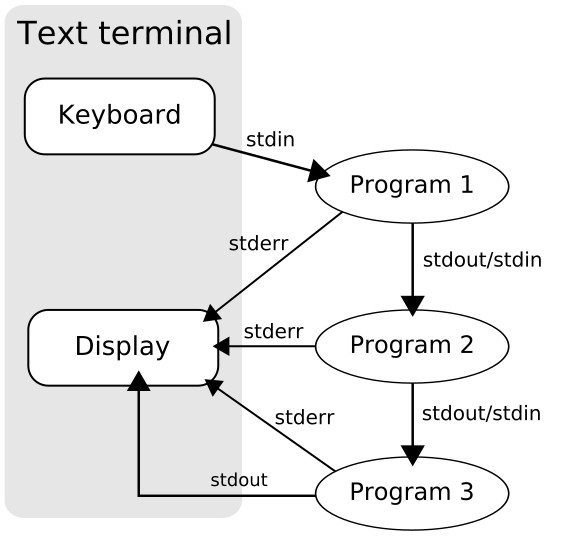
\includegraphics[width=0.3\textwidth]
		{images/Pipeline.jpg}
	\caption{Unix Pipeline Mechanism}
	\label{fig:unixPipe}
\end{figure}

For more explanation, we provide a simple test case. Consider two different program,
{\it factor} and {\it calc}. Given a single argument, {\it factor} will show you all 
factors of a number. Given also a single argument, {\it calc} will show you the result 
of an arithmetic operation. Listing ~\ref{factorAndCalc} shows the outputs of both commands

\begin{lstlisting}[caption=Usage of factor and calc, label=factorAndCalc, language=bash, basicstyle=\small, breaklines=true]
#! factor 20
20: 2 2 5

#! calc 7+3 
10
\end{lstlisting}

Unix pipe mechanism allows you to combine those two programs. For example, if you
want the output of {\it calc} become the input of {\it factor}, you can use pipe
command as shown in listing ~\ref{unnamedPipeExample}

\begin{lstlisting}[caption=Unnamed pipe example, label=unnamedPipeExample, language=bash, basicstyle=\small, breaklines=true]
#! calc 7+3 | factor
10: 2 5
\end{lstlisting}

Beside of it's high availability and simplicity, UNIX pipe also supports parallel
processing through named-pipe mechanism. The named-pipe mechanism can be used to 
provide cheap parallel processing \cite{conway2003parallel}. 

In listing ~\ref{namedPipeExample} we show a simple named-pipe mechanism. First, we make
a named pipe called {\it backpipe} by using {\it mkfifo} command. Next, we redirect
standard output of {\it calc} and {\it factor} into {\it backpipe}. Finally, we show
the content of the {\it backpipe} by using {\it cat} command.

\begin{lstlisting}[caption=Named pipe example, label=namedPipeExample, language=bash, basicstyle=\small, breaklines=true]
#! mkfifo backpipe 

#! calc 7+3 > backpipe | factor 20 > backpipe | cat backpipe
10
2 2 5
\end{lstlisting}

Although pipe mechanism provides high availability and capability, 
it has several limitations. For example, named-pipe needs external file as temporary 
container. The external file has to be deleted once the operation performed. 
This approach is not straight forward, thus, some efforts eeded in order to 
to build a working named-pipe based computation. 

For simple use cases involving a single computer, pipe mechanism is quite ideal. 
However, at some point, when the program become more complicated, memory sharing 
and network access is needed. Using a mere pipe mechanism to support those 
requirement needs a lot of efforts. Although it is possible, the readability of
the script is going to be severely reduced.


\subsection{CORBA}

From CORBA official website, CORBA is defined as standard created by the Object 
Management Group designed to facilitate the communication of systems 
that are deployed on diverse platforms \cite{corba}. CORBA 1.0 was released on August 
1991. The last version, CORBA 3.3 was released on November 2012 \cite{corbaspec}.
CORBA is heavily affected by object oriented paradigm.

The main component of CORBA is the Object Request Broker (ORB). ORB act as bridge 
between client and service provider. The service provider (server) provide an 
implementation of an object. While the client can be a user interface that depend on
the service provided by the server. Both, client and server needs to agree about the
object structure. This agreement is written in an Interface Description Language (IDL).
The IDL in server side is called skeleton, while the IDL in client side is called stub.

\begin{figure}
	\centering
	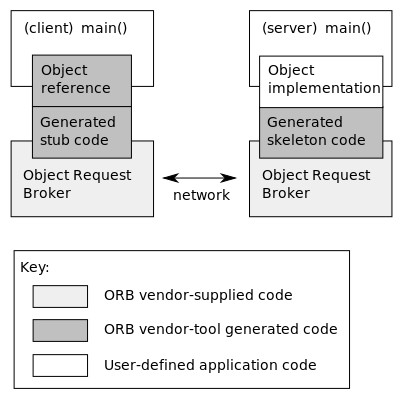
\includegraphics[width=0.3\textwidth]
		{images/Orb.jpg}
	\caption{Object Request Broker}
	\label{fig:orb}
\end{figure}

Figure ~\ref{fig:orb} shows the interaction between ORB, server, and client.
IDL can be written in Java, C++, or any other language, depend on the implementation of
the ORB.

An IDL example is shown in listing ~\ref{corbaIDLExample}.

\begin{lstlisting}[caption=CORBA IDL Example in C++, label=corbaIDLExample, language=c, basicstyle=\small, breaklines=true]
module Finance {
  typedef sequence<string> StringSeq;
  struct AccountDetails {
    string     name;
    StringSeq  address;
    long       account_number;
    double     current_balance;
  };
  exception insufficientFunds { };
  interface Account {
    void deposit(in double amount);
    void withdraw(in double amount) raises(insufficientFunds);
    readonly attribute AccountDetails details;
  };
};
\end{lstlisting}

Compared to UNIX Pipe, CORBA is more feature rich and complex. The developer needs to 
embrace OOP paradigm as well as being familiar with IDL and the CORBA architecture. 
Despite of it's language agnoticism, some non OOP language (e.g: Matlab and GNU Octave) 
is not supported by CORBA \cite{feilhauer2016def}. CORBA also suffer of several 
criticism \cite{henning2006rise}. Even OOP as the foundation of CORBA, also face several 
critics \cite{hadar2013intuition} regardless of it's popularity.


\subsection{XML-RPC, SOAP, and JSON-RPC}

XML-RPC is a spec and a set of implementations that allow software running on 
disparate operating systems, running in different environments to make procedure 
calls over the Internet. XML-RPC using HTTP as the transport and XML as the encoding.
It is designed to be as simple as possible, while allowing complex data structures to 
be transmitted, processed and returned \cite{xmlrpc}.

SOAP stands for Simple Object Access Protocol. SOAP is a lightweight protocol 
intended for exchanging structured information in a decentralized, distributed 
environment \cite{soap}. SOAP was built on top of XML-RPC. It uses XML format as 
well as HTTP protocol.

JSON-RPC is lightweight remote procedure call protocol similar to XML-RPC 
\cite{jsonrpc}. The main difference between XML-RPC and JSON-RPC is the data transfer
format. In most cases, JSON is more lightweight compared to XML.

XML-RPC, SOAP, and JSON-RPC are heavily depend on HTTP for inter-process-communication 
protocol. This is ideal for client-server architecture as HTTP is quite common and
easy to be implemented.

Those three methods are basically another implementation of RPC (Remote Procedure Call). 
Compared to CORBA, these three methods are more flexible. With the exception of SOAP,
they don't enforce developer to embrace OOP paradigm.

In terms of language agnoticism, XML-RPC and JSON-RPC support any language that can
access HTTP and parse/create the data format. However, in order to use these protocols,
a developer should be aware that the components they built will works as a part of the
bigger system. Tools or programs that were built without this consideration will need
some adjustment or additional layers in order to make them works with the protocol.
For example, using {\it{factor}} or {\it{calc}} as components of XML-RPC might require
developer to build another program to catch the output and wrap it in XML envelope.

\subsection{DEF}

DEF - A programming language agnostic framework and execution environment 
for the parallel execution of library routines \cite{feilhauer2016def}. 
DEF focus on parallel processing by enabling shared memory and message passing. 
DEF needs several components, using JSON as data exchange format. 
Compared to CORBA, Matlab, and Parallel Fortran, DEF is better in term of 
parallelism and language agnosticism. CORBA for example, doesn't support matlab and 
octave \cite{feilhauer2016def}. 

However, DEF still depend on HTTP for inter process communication. Consequently, 
in order to build DEF architecture, a web server is needed. Also, the developer needs 
to make sure that each components aware of the architecture. As in CORBA, XML-RPC, 
SOAP, and JSON-RPC, additional layer might be needed to make use of old components.

\subsection{Beaker Notebook}

Beaker Notebook \cite{beakernotebook} is also considered as an interesting 
approach of CBSE. The platform was developed by Two Sigma Open Source and 
mainly used for research use. 

Beaker provides native autotranslation that lets a developer declare specific 
variables in a cell in one language, then access these seamlessly in a 
different cell and language.

Using Beaker Notebook, a developer can access a global inter-language variable
from different cells. The cells can also be written in any language supported.

For example, in listing ~\ref{beakerPython}, we create a 6 by 4 table populated with
random numbers. The table is then saved as global variable df. 
Later in listing ~\ref{beakerR}, we load the data and show it.

\begin{lstlisting}[caption=Beaker Python Cell Example, label=beakerPython, language=python, basicstyle=\small, breaklines=true]
import pandas
beaker.df = pandas.DataFrame(np.random.randn(6, 4), columns = list('ABCD'))
\end{lstlisting}

\begin{lstlisting}[caption=Beaker R Cell Example, label=beakerR, language=R, basicstyle=\small, breaklines=true]
beaker::get('df')
\end{lstlisting}

Beaker notebook is good for prototyping. It also has a very simple API compared to
CORBA or XML-RPC. However, it still require the developer to add additional layer
in order to use old components like {\it factor} or {\it calc}


\section{Chimera Architecture}

From the previous section we conclude that Unix Pipe Mechanism was the simplest one
despite of it's lack of features. We also notice that Beaker Notebook's like memory-
sharing mechanism is much simpler compared to CORBA and other network-based protocols.

Our goal is to make a very simple framework that is truly language agnostic. A framework
that also play nice with old components and not enforce developer to embrace any 
particular programming paradigm. Also, we try to avoid making unnecessary new standard.
By make use of tecnologies most developers familiar with, we hope the adaptation is
going to be easier.

We assume that most programming languages are supporting command line interface and
command line arguments. By creating a framework that depend on command line protocol,
we aim on maximum language agnosticism with less effort.

In figure ~\ref{fig:chimeraArchitecture} we show the architecture of Chimera. Suppose
{\it Program1} and {\it Program2} should run in parallel, and {\it Program3} should be
executed once {\it Program1} and {\it Program2} finished.

Chimera architecture contains of several parts. The Chimera Core is the main component 
responsible for orchestrating external programs into a single process flow. 
Chimera core can access Temporary Memory which is no other than a JSON Object placed in
memory. All external program's input and output are copied into this JSON Object.
The process flow itself is written in a YAML Chain File. YAML is a common format for
configuration. YAML depends on indentation and whitespace, making the format easily 
readable. Using these three components, Chimera is able to do everything UNIX Pipe can. 
In fact, developers can even define UNIX Pipe inside Chimera.

The other two components are Chimera-Service and Chimera-Sender. These two components
are responsible for HTTP communication. Bringing the entire framework into distributed
environment.

In figure ~\ref{fig:chimeraArchitecture}, the process started when the user ask Chimera 
to execute the process. User should provide the YAML file location and the process's
inputs. After getting a request from user, Chimera will read the YAML file, retrieving
it's content, and initiating global variables in Temporary memory. The framework then
executing external programs sequentially or parallelly, depend on the content of the
YAML file.

If the external programs are located in the same computer, Chimera-Core will execute the
programs and provide the required stdin parameters. The stdin parameters are taken from
Temporary Memory. After the program executed successfully, Chimera-Core will read the 
stdout and save it into Temporary Memory for further process.

If the programs are located in the different computer, the user should provide
invocation of Chimera-Sender. Chimera-Sender will contact Chimera-Service to run 
Chimera-Core remotely. Once the process completec, Chimera-Service will send the
response into Chimera-Sender. At last, Chimera-Sender will send the response back to
the local Chimera-Core.

At the end of the process, Chimera will return the output of those chain-processes to 
the user.

\begin{figure*}
	\centering
	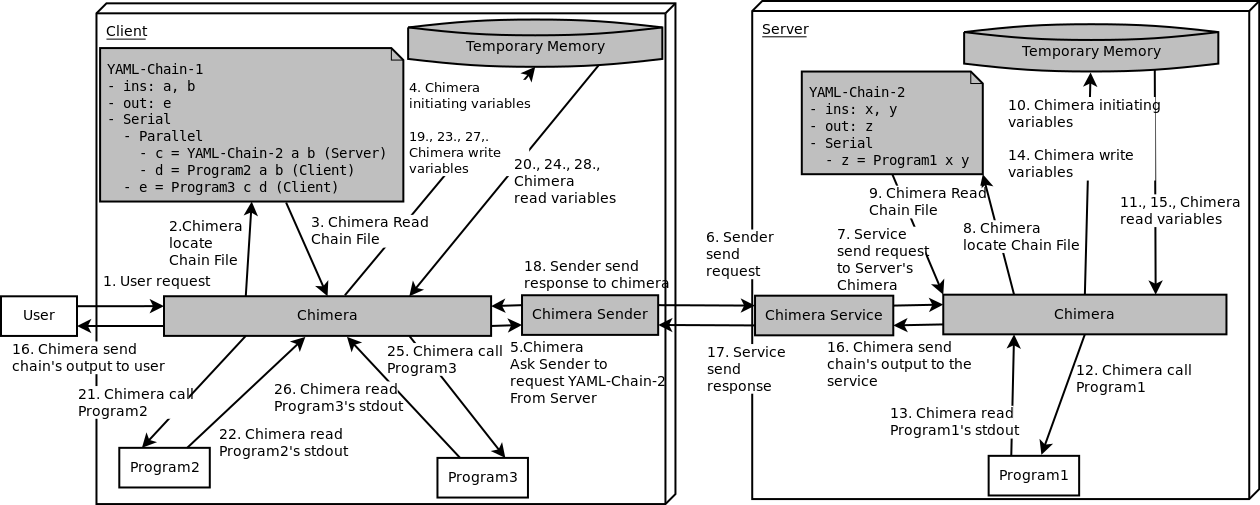
\includegraphics[width=1.0\textwidth]
		{images/chimera.png}
	\caption{Architecture of Chimera}
	\label{fig:chimeraArchitecture}
\end{figure*}

\section{Chimera Technical Implementation}

We already publish Chimera as NPM package. It is accessible through 
https://www.npmjs.com/package/chimera-framework.


\subsection{Node.js and NPM As Chimera's Foundation}

Chimera is written in Node.js. Node.js itself is a JavaScript runtime built on Chrome's 
V8 JavaScript engine. Node.js uses an event-driven, non-blocking I/O model that makes it 
lightweight and efficient \cite{nodejs}. Compared to Python and PHP, Node.js has an 
overall better performance \cite{lei2014performance}. Node.js is also available for
Windows, Linux, and Mac.

Node.js has a package-manager named NPM (Node Package Manager). This allows developers
to use libraries that have already been written by other developers. Chimera depend on 
several packages:

\begin{itemize}
    \item async
    \item express
    \item fs-extra
    \item http
    \item js-yaml
    \item node-cmd
    \item path
    \item process
    \item querystring
\end{itemize}

Async package is used to develop the control flow since Node.js has non-blocking
mechanism. Express is used to build Chimera-Service. Express allows us to catch request
and send appropriate response. We also use fs-extra in order to do file operations.
Http and querystring is used to build Chimera-Sender. We also need several functionality
provided by node-cmd in order to execute other programs through CLI mechanism.
Js-yaml is used for YAML parsing. At last, we need path and process to determine 
absolute path of a file as well as changing directory and retrieving input arguments.

\subsection{YAML for Defining Chain}

YAML (YAML Ain't Markup Language) is a human friendly data serialization standard for 
all programming languages \cite{yaml}. YAML standard was built in 2001. Unlike JSON,
YAML depends heavily on indentation. Although the size is bigger compared to JSON, YAML
is very readable and commonly used for configuration.

At the beginning Chimera's chain file was intended to use JSON format. However, we realize 
that using JSON format might not be a good decision since the developers has to be very 
careful with comma and curly braces. Another disadvantage
of JSON is it doesn't provide any intuitive way to add comments, which is quite
essential in writing algorithms.

Let's consider we have several programs written in Python, Java, PHP, and Javascript. 
Each of them takes 2 arguments, do simple arithmetic operation, and return a single output. 
Given a and b, you want to calculate ((a+b) * (a-b)) + a.

You can write the process as follow:

{\it f = ((a+b) * (a-b)) + a}

You can then divide this process into several sub-processes:

\begin{itemize}
    \item Process 1: c = a + b
    \item Process 2: d = a - b
    \item Process 3: e = c * d
    \item Process 4: f = e + a
\end{itemize}

Process 1 and process 2 will be executed in parallel since they are independent to each other. 
You don't need to solve process 1 in order to do process 2 and vice versa.

After Process 1 and process 2 finished, process 3 and process 4 should be executed in serial. 
Process 3 depend on process 1 and 2, while process 4 depend on process 3

Listing ~\ref{yamlChainExample} is the example of our YAML formatted chain file.

\begin{lstlisting}[caption=YAML Chain Example, label=yamlChainExample, language=yaml, basicstyle=\small, breaklines=true]
ins: a,b # The inputs of main process 
out: f # The outputs of main process 
series:
  # Process 1 and 2 
  - parallel:
      # Process 1 (in Python) 
      - ins: a, b
        out: c
        command: python programs/add.py
      - series: # Process 2 (in Java) 
          # First, compile the source  
          - javac programs/Substract.java
          # then run the program 
          - ins: a, b
            out: d
            command: java -cp programs Substract
  # Process 3 (in PHP) 
  - ins: c, d
    out: e
    command: php programs/multiply.php
  # Process 4 (in Javascript) 
  - ins: e, a
    out: f
    command: node programs/add.js
\end{lstlisting}

Semantically, each node in the YAML contains of {\it ins} and {\it out }, assuming
every program can has more than one inputs but only provide single output. The last
element of the node is either {\it command}, {\it parallel}, or {\it series}. 
If the process has no other sub-process, {\it command} is used. Otherwise, if the
process contains another sub-process, {\it parallel} or {\it series} is used depend
on the desired execution flow. The best practice is, when two or more processes
doesn't depend on each other, parallel flow is recommended.

For convenience, we also provide single-line shorthand for {\it ins}, {\it out}, 
and {\it command}. {\it ins} should be written inside parantheses, while {\it ->}
act as separator between {\it ins}, {\it command}, and {\it output}. For example,
Listing  ~\ref{yamlShort} is equal to Listing ~\ref{yamlChainExample}.

\begin{lstlisting}[caption=YAML Chain With Shorthand, label=yamlShort, language=yaml, basicstyle=\small, breaklines=true]
ins: a,b # The inputs of main process 
out: f # The outputs of main process 
series:
  # Process 1 and 2 
  - parallel:
      # Process 1 (in Python) 
      - (a,b) -> python programs/add.py -> c
      - series: # Process 2 (in Java) 
          # First, compile the source  
          - javac programs/Substract.java
          # then run the program 
          - (a,b) -> java -cp programs Substract -> d
  # Process 3 (in PHP) 
  - (c,d) -> php programs/multiply.php -> e
  # Process 4 (in Javascript) 
  - (e,a) -> node programs/add.js -> f
\end{lstlisting}


\subsection{JSON Format for Temporary Global Storage and Data Transfer}

As we use Node.js, it is natural to also use Javascript Object Notation as Chimera's
global storage and network data transfer. JSON (JavaScript Object Notation) is a 
lightweight data-interchange format \cite{json}.

Once the YAML Chain File parsed, Chimera will create several variables in {\it name : 
value} pairs. For example, after loading YAML in listing ~\ref{yamlChainExample}, the
global variables will contains JSON object as in listing ~\ref{jsonStorageInitial}.

As the sub-process executed, several others variables will be added as needed. At the
end of the process, the global storage will contains a, b, c, d, e, and f.

\begin{lstlisting}[caption=Initial content of JSON Storage, label=jsonStorageInitial, language=json, basicstyle=\small, breaklines=true]
{
    "a" : 0,
    "b" : 0,
    "f" : 0,
}
\end{lstlisting}

Not only for temporary storage, we also use JSON for data transfer between 
Chimera-Sender and Chimera-Service. The data sent to Chimera-Service is shown in Listing
~\ref{jsonRequest}, while the data received by Chimera-Sender is shown in Listing
~\ref{jsonResponse}.

The JSON request contains 2 keys. The "chain" is to 
indicate the remote YAML chain file location, while "input" contains array of inputs.

The JSON response contains 3 keys. The {\it success} key is to indicate
whether the request succeed or failed. {\it errorMessage} contains the error message, and
{\it response} is the response from the server.

\begin{lstlisting}[caption=JSON Request, label=jsonRequest, language=json, basicstyle=\small, breaklines=true] 
{
    "chain" : "remote-chain-file.yaml",
    "input" : [],
}
\end{lstlisting}

\begin{lstlisting}[caption=JSON Response, label=jsonResponse, language=json, basicstyle=\small, breaklines=true]
{
    "success" : true,
    "errorMessage" : "",
    "response" : "",
}
\end{lstlisting}


\subsection{Utilities}

Several utilities were built as component of Chimera Framework.

\begin{itemize}
    \item Chimera-core
    \item Chimera-eisn
    \item Chimera-serve
    \item Chimera-send
\end{itemize}

Chimera-core is the main component of the framework. User can invoke chimera by
executing {\it chimera your-chain-file.yaml [input1 [input2] ... ]}. For convenience,
some shorthand are also provided. For example, you can also call 
{\it chimera "command:cal"} or even {\it chimera "cal"}.

Chimera-eisn take at least 3 input arguments. The first and the second argument should
be file name, while the third arguments should be the command. The command will only
be executed when the first argument's modification date is newer than the second 
argument. EISN itself is stands for "Execute If Source Newer". This is useful if user
want to use source code of compiled language as an argument. 
The typical example is shown in Listing ~\ref{chimeraEisn}

\begin{lstlisting}[caption=Chimera-eisn usage example, label=chimeraEisn, language=yaml, basicstyle=\small, breaklines=true]
ins: a, b
out: c
series:
    - chimera-eisn add.java add.class javac add
    - ins: a, b
      out: c
      command: java add
\end{lstlisting}

Chimera-serve is a utility to let several chain file being served by a computer.
The typical usage of chimera-serve is:

{\it TIMEOUT=5000 PUBLISHED=. chimera-serve}

The first two statements are used to define timeout and published directory. Dot means
current directory. All chain file in published directory is then accessible over
the network.

Chimera-send is a utility to access chimera service.
The typical usage of chimera-send is: 

{\it TIMEOUT=5000 chimera-send remoute-chain-file.yaml [input1 [input2] ... ]}


\section{Test}

We use Listing ~\ref{distributedParallelYaml} in order to test that Chimera works
in parallel and distributed environment.

\begin{lstlisting}[caption=Distributed and Parallel YAML-chain Scenario, label=distributedParallelYaml, language=yaml, basicstyle=\small, breaklines=true]
ins: a,b,server
out: e
vars:
  server_chain: tests/chain-minimal.yaml 
verbose: true
series:
  - parallel:
      # Process 1
      - (a,b) -> php programs/add.php -> c
      # Process 2
      - (server, server_chain, a,b) -> chimera-send -> d
  # Process 3
  - (c,d) -> node programs/add.js -> e
\end{lstlisting}

The chain contains of 3 processes. Process 1 and process 2 will be executed in parallel.
After process 1 and process 2 finished, process 3 will be executed. Unlike process 1 and
process 3, process 2 will run on the server.

On the server side, we execute {\it chimera-serve} so that it will listen to client's request
and giving response as necessary.

On the client side, we execute {\it chimera tests/chain-distributed.yaml 4 5 http://localhost:3000}

Client log is shown on ~\ref{clientLog} 

\begin{lstlisting}[caption=Client Log, label=clientLog, language=bash, basicstyle=\small, breaklines=true]
START [php programs/add.php "4" "5"] AT    : 15,395,587,568,188
START [chimera-send "http://localhost:3000" "tests/chain-minimal.yaml" "4" "5"] AT    : 15,395,607,233,624
END   [php programs/add.php "4" "5"] AT    : 15,395,641,517,534
TAKES 53,905,697 NS
END   [chimera-send "http://localhost:3000" "tests/chain-minimal.yaml" "4" "5"] AT    : 15,396,103,823,215
TAKES 496,566,143 NS
START [node programs/add.js "9" "-5"] AT    : 15,396,105,155,463
END   [node programs/add.js "9" "-5"] AT    : 15,396,187,724,022
TAKES 82,541,434 NS
4
\end{lstlisting}

From the log, we can see that the second process on client side was executed before the first process finished.
However, the third process didn't started before the second process started. Process 2 output was taken from the
server's response.

\section{Conclusion}

In this paper, we have developed Chimera, a simple language agnostic CBSE Framework. 
The framework is quite simple, yet powerful enough for distributed and parallel computation.

Old UNIX commands like {\it calc} and {\it factor} work perfectly under the framework.
No additional layer is needed.

%\appendices
%\section{Proof of the First Zonklar Equation}

% use section* for acknowledgement
\section*{Acknowledgment}

The authors would like to thank Sonny Setiawan, Satriyo Wibowo, and Dani Devito for
their suggestions and opinions. Sonny Setiawan is a Marketing Business Analyst in Malang.
Satriyo Wibowo is an IT professional in Jakarta. Dani Devito is an IT student in Malang.

% Can use something like this to put references on a page
% by themselves when using endfloat and the captionsoff option.
\ifCLASSOPTIONcaptionsoff
  \newpage
\fi

\bibliographystyle{IEEEtran}
\bibliography{./citation}

% that's all folks
\end{document}

